% !TeX document-id = {f5eab2f7-1326-43b3-ac0e-350c2acbded8}

% !TeX TXS-program:compile = txs:///pdflatex/[--shell-escape]

\documentclass[a4paper, fontsize=11pt, parskip=half, twoside]{scrreprt}

\usepackage[utf8]{inputenc}
\usepackage[T1]{fontenc}   
\usepackage{graphicx}       
\usepackage[english, ngerman]{babel}
\usepackage{csquotes} % for displaying quotes  
\usepackage{acronym}
\usepackage{eurosym}
\usepackage[linktocpage=true]{hyperref}
\usepackage{xurl}
\usepackage[bindingoffset=8mm]{geometry}
\usepackage{caption}
\captionsetup{format=hang, justification=raggedright}
\usepackage[style=authoryear, backend=biber]{biblatex}
\usepackage{float}
\usepackage{rotating}
\usepackage{amsmath}
\usepackage{amssymb}
\usepackage{outlines} % for nested lists
\usepackage{tikz} % for drawing
\usepackage{microtype} % improve micro typography for better distribution
\usepackage{minted} % for source code
\usepackage{caption} % caption for e.g. figures
\usepackage{subcaption} % captions for multiple figures
\usepackage{datetime} % for custom dates
\usepackage[german]{cleveref} % clever refs - set labels as always (\label{fig:hello}), \cref{fig:hello}
\usepackage[onehalfspacing]{setspace} % 1.5x line space

% adds generic commands for degree, ohm, ..
\usepackage{textcomp}
\usepackage{gensymb}

\usepackage{todonotes}

% custom commands
\renewcommand{\listingscaption}{Quellcode}
\renewcommand{\listoflistingscaption}{Quellcodeverzeichnis}
\providecommand*{\listingautorefname}{Quellcode}

\definecolor{bg}{rgb}{0.93, 0.93, 0.93}
\setminted{
	autogobble, 
	tabsize=4, 
	numbers=left,
	numbersep=15pt,
	bgcolor=bg,
	fontsize=\footnotesize
}
\renewcommand{\fcolorbox}[4][]{#4} % "disables" syntax errores in minted code blocks 

% define date variable for whole doc
% use \displaydate{date} where needed to insert this date

\newdate{date}{01}{07}{2023}
\date{\displaydate{date}}

% add zotero file for citations
\addbibresource{reference.bib}

\begin{document}
	
	\thispagestyle{empty}
	
	\cleardoublepage   % force output to a right page
	\thispagestyle{empty}
	\begin{titlepage}
		\begin{flushright}
			
\includegraphics[width=0.4\linewidth]{assets/Logo-A3.jpg}
		\end{flushright}
		
		\begin{flushleft}
			\section*{Integration eines Feature-orientierten Testsystems in den Entwicklungszyklus technischer Systeme}
			%\subsection*{\papersubtitle}
			\vspace{1cm}
			
			\vspace{0.5cm}
			Bachelorarbeit\newline
			zum Erlangen des akademischen Grades\newline
			
			\vspace{0.5cm}
			\textbf{Bachelor of Science in Engineering (BSc)}
			
			\vspace{1cm}
			Fachhochschule Vorarlberg\newline
			Informatik - Software and Information Engineering\newline
			
			\vspace{0.5cm}
			Betreut von\newline
			Dipl.-Ing. Dr. techn. Ralph Hoch
			
			\vspace{0.5cm} 
			Vorgelegt von\newline
			Marco Prescher	
			
			\vspace{0.5cm}
			Dornbirn, am \displaydate{date}
		\end{flushleft}
	\end{titlepage}
	
	% Kurzreferat
	\newpage
	\section*{Kurzreferat}
	\subsection*{Integration eines Feature-orientierten Testsystems in den Entwicklungszyklus technischer Systeme}
	
	Die Entwicklung technischer Systeme ist ein komplexer und kostspieliger Prozess. 
	Daher ist es wichtig, dass die Produkte vor der Auslieferung an den Kunden gezielt und sorgfältig getestet werden. 
	Dies wird durch Zeitdruck und Deadlines oftmals vernachlässigt, oder nur unzureichend durchgeführt. 
	Mit einem gut strukturierten Testplan kann dieses Risiko allerdings minimiert werden, und die Durchführung der Tests mit dem Produktentwicklungszyklus integriert werden. 
	Dadurch kann stabile Hardware sowie effiziente und gut strukturierte Software ohne große Verzögerung an den Kunden ausgeliefert werden.
	
	Durch Methodiken wie zum Beispiel Feature-orientierte Entwicklung ist es möglich, dass bestimmte Features vor dem Release der Produkte abgenommen und getestet werden müssen. 
	Das wiederum ermöglicht, dass neu implementierte Features gründlich getestet werden und somit zu einer hohen Qualität beitragen.
	
	Dies kann erreicht werden, indem Features strukturiert in einer Datenbank eingepflegt werden. 
	Ein auf diesen Featurebeschreibungen basierendes System kann die automatische Testdurchführung unterstützen, gezielt Tests für einzelne Features durchführen und deren Abnahme beschleunigen. 
	Dadurch kann der Testaufwand verringert und den Entwicklern ein fokussiertes Feedback vermittelt werden.
	
	\newpage
	\section*{Abstract}
	\subsection*{Integrating a feature-oriented testing system into the development cycle of technical systems}
	
	The development of technical systems is a complex and costly process. 
	Therefore, it is important that products are thoroughly tested before delivery to the customer. 
	However, this is often neglected or done insufficiently due to time pressure and deadlines. 
	A well-structured test plan can minimize this risk and integrate the testing process into the product development cycle. 
	This allows stable hardware and efficient, well-structured software to be delivered to the customer without significant delays.
	
	Using techniques such as feature-oriented development, certain features must be accepted and tested before the product release. 
	This in turn allows newly implemented features to be thoroughly tested and contribute to high quality. 
	
	This can be achieved by structuring features in a database. 
	A system based on these feature descriptions can support automatic testing, conduct targeted tests for individual features, and accelerate their acceptance. 
	This reduces testing effort and provides focused feedback to the developers.
	
	% Inhaltsverzeichnis
	\cleardoublepage   % force output to a right page
	\setcounter{tocdepth}{2}
	\setcounter{secnumdepth}{4}
	\tableofcontents
	
	% Abbildungsverzeichnis
	\clearpage
	\phantomsection
	\addcontentsline{toc}{chapter}{Abbildungsverzeichnis}
	\listoffigures
	
	% Quellcodeverzeichnis
	\clearpage
	\phantomsection
	\addcontentsline{toc}{chapter}{Quellcodeverzeichnis}
	\listoflistings
	
	% Abkürzungsverzeichnis
	\clearpage
	\phantomsection
	\addcontentsline{toc}{chapter}{Abkürzungsverzeichnis}
	\section*{Abkürzungsverzeichnis}
	\begin{acronym}
		\acro{API}{Application Programming Interface}
		\acro{JSON}{JavaScript Object Notation}
		\acro{TCMS}{Test Case Management System}
		\acro{TDD}{Test Driven Development}
		\acro{EF}{Entity Framework}
		\acro{ORM}{Object Relational Mapping}
		\acro{OAS}{OpenAPI Spezifikation}
		\acro{HTTP}{Hypertext Transfer Protocol}
		\acro{MVP}{Minimum Viable Product}
		\acro{UI}{User Interface}
		\acro{DDD}{Domain Driven Design}
		\acro{DHCP}{Dynamic Host Configuration Protocol}
		\acro{GI}{Gantner Instruments}
		\acro{TAS}{Test Automation System}
		\acro{IDE}{Integrated Development Environment}
	
		\acrodefplural{TCMS}{Test Case Management Systeme}
	\end{acronym}
	
	\clearpage
	\section*{Danksagung}
	Ich möchte mich aufrichtig bei Ralph Hoch, der Firma Gantner Instruments und allen Mitarbeitenden bedanken, die mir bei der Vollendung dieser Arbeit geholfen haben. 
	Ihre Unterstützung und Expertise waren von unschätzbarem Wert und haben zum erfolgreichen Abschluss dieses Projekts beigetragen. 
	Vielen Dank für Ihre harte Arbeit und Ihr Engagement. 
	Ich schätze Ihre Zusammenarbeit sehr.
	
	
	
	\clearpage
	\chapter{Einleitung}
	
	\begin{flushright}
		\rightskip=8cm\textit{``Time is money.''} \\
		\vspace{.2em}
		\rightskip=6cm--- \textcite{franklin_advice_1748}
	\end{flushright}

	In der Softwareentwicklung kann es durch Fehler und Mängel zu Verzögerungen und dadurch zu Verlusten kommen.
	Deswegen wurde in Zusammenarbeit mit der Firma \acfi{GI} geplant ein \acfi{TCMS} zu entwickeln.
	Diese Arbeit fokussiert sich daher auf die Implementierung von einem \ac{TCMS} und vergleicht verschiedene vorhandene Lösungen.
	
	
	\section{Motivation} \label{sec:motivation}
	Die Entwicklung technischer Systeme ist ein komplexer Prozess, der eine hohe Qualität erfordert, um den Anforderungen der Kunden gerecht zu werden. 
	Damit diese Qualität auch gewährleistet wird, müssen Fehler sowie Mängel identifiziert und ausgebessert werden. 
	Ein \ac{TCMS} bietet eine Lösung, um diesen Prozess zu vereinfachen und effektiver zu gestalten. 
	Durch die Verwendung eines \ac{TCMS} können Angestellte aus verschiedenen Abteilungen, wie z.B. der Software-, Hardware-, Support- oder Marketingabteilung, die Qualität des Produkts gemeinsam verbessern. 
	
	\section{Problemstellung}
	Durch die von \autoref{sec:motivation} angesprochene Komplexität technischer Systeme ist bekannt, dass Fehler, die erst spät im Entwicklungsprozess entdeckt werden, viel kostspieliger zu beheben sind als Fehler, die frühzeitig identifiziert und behoben werden. \textcite{westland_cost_2002}
	
	Infolgedessen suchen Unternehmen nach Lösungen, um den Testprozess effektiver zu gestalten und Fehler früher im Entwicklungszyklus zu identifizieren. 
	\ac{TCMS} bietet eine solche Lösung, indem es Entwicklern und Testern ermöglicht, Testfälle effizient zu planen und zu verwalten sowie Testergebnisse zu erfassen, darzustellen und somit auch zu verfolgen. 
	Obwohl \ac{TCMS} in der Industrie weit verbreitet sind und es einige fertige Lösungen gibt, gibt es jedoch nicht immer die perfekte Lösung um ein bestehendes \ac{TCMS} für das eigene Projekt anzuwenden. 
	Insbesondere gibt es Bedenken hinsichtlich der Anwendbarkeit und Integration von einem schon bestehendem \ac{TCMS}, da dieses System auch mit internen Tools kommunizieren können muss.
	Diese Probleme stellen Hindernisse dar, die die Einführung von \ac{TCMS} in einem Unternehmen erschweren. 
	Diese Arbeit beschäftigt sich mit diesen Problemen und untersucht, wie ein \ac{TCMS} effektiv eingesetzt werden kann.
	
	\section{Zielsetzung}
	Das Ziel dieser Arbeit ist es, die Verwendung von \ac{TCMS} zu untersuchen und zu bewerten. 
	Zudem ein auf unser eigenes Produkt angepasstes \ac{TCMS} zu entwickeln. 
	Hiermit ergeben sich drei relevante fragen:
	
	\begin{itemize}
		\item Wie kann man Features, Testfälle und Testimplementierungen beschreiben? 
		\item Wie in Datenbank schreiben und lesen? 
		\item Wie mit Testläufen verknüpfen?
	\end{itemize}
	
	Insbesondere möchten wir die folgenden Ziele erreichen:
	
	\begin{itemize}
		\item Die Vor- und Nachteile der Verwendung von einem \ac{TCMS} zu identifizieren und zu analysieren.
		\item Empfehlungen für die erfolgreiche Implementierung eines \ac{TCMS} in der Softwareentwicklung zu geben, einschließlich der Identifizierung bewährter Praktiken.
	\end{itemize}
	
	Durch die Erfüllung dieser Ziele wird diese Arbeit dazu beitragen, das Verständnis für die Verwendung von einem \ac{TCMS} in der Produktentwicklung zu verbessern und Unternehmen dabei zu unterstützen, den Testprozess zu optimieren und die Qualität ihrer Produkte zu verbessern.
	
	
	
	\chapter{Stand des Wissens}
	Dieses Kapitel gibt einen Überblick über den aktuellen Stand der Technik von Testarten, \ac{TCMS} sowie deren Verwendung und Integration mit bestehenden Systemen. 
	Weiters werden Technologien, auf denen das in dieser Arbeit entwickelte \ac{TCMS} aufbaut, beschrieben.
	
	\section{Testarten} \label{sec:testtypes}
	Während der Entwicklung eines Produkts kommen unterschiedliche Testarten zum Einsatz. 
	\textcite{atlassian_unterschiedlichen_nodate} beschreibt sieben unterschiedliche Testverfahren die je nachdem andere Aspekte eines Produkts testen.
	In \textcite{noauthor_software_nodate} wird beschreiben, dass dabei zwischen \emph{Funktionalen} und \emph{Nicht-Funktionalen} Tests unterschieden werden.
	Zu der funktionalen Testfamilie zählen beispielsweise Unit-Tests und Integrationstests.
	Nicht funktionale Testarten sind beispielsweise Leistung, Last und Stresstests sowie Usability-Tests zu den nicht funktionalen Testfamilie gehören.
	
	Ein paar der am häufigsten vorkommenden Testarten sind:
	
	\begin{itemize}
		\item Unit-Tests
		\item Integrationstests
		\item Funktionstests
		\item Leistungstests
	\end{itemize}

	Um eine Testabdeckung sicherzustellen und den allgemeinen Testprozess zu optimieren werden \ac{TCMS} eingesetzt. 
	Diese Systeme bieten eine zentrale Plattform zur Verwaltung von Testfällen, wo Tests, die für ein Release oder Produkt erforderlich sind, erstellt und dokumentiert werden können (Siehe \autoref{sec:tcms}). 
	
	\textcite{ammann_introduction_2016}
	
	\subsection{Unit-Tests}
	Im Allgemeinen sind Unit-Tests Tests die beispielsweise Methoden einer Klasse mit unterschiedlichen Parametern testet. 
	Sie sind automatisierbar und können von einer Continuos-Integration-Pipeline durchgeführt werden. 
	Diese Tests ermöglichen eine kontinuierliche Überprüfung der Funktionsfähigkeit des Produkts im Entwicklungsprozess und unterstützen das frühzeitige Finden von Fehlern.
	
	\subsection{Integrationstests}
	Integrationstests sind Tests, die sicherzustellen, dass verschiedene Module oder Services, problemlos miteinander interagieren können. 
	Durch diese Tests kann die Funktionalität einzelner Teile der Anwendung überprüft werden, wie beispielsweise die Interaktion mit einer Datenbank oder der Zusammenarbeit von Microservices.
	
	\subsection{Funktionstests}
	Funktionstests werden integriert, um ausschließlich Ergebnisse einer gegebenen Funktion zu überprüfen. Dabei werden Spezifikation vor der Testausführung festgelegt und diese dann mit den Ergebnissen verglichen.
	
	Während Integrationstests beispielsweise nur prüfen, ob Datenbankabfragen generell möglich sind, wird bei einem Funktionstest ein bestimmter Wert aus der Datenbank abgerufen und dieser mit den angegebenen Spezifikationen geprüft.
	
	\subsection{Leistungstests}
	Leistungstests prüfen das Verhalten eines Systems unter verschiedenen Lastprofilen zu überprüfen. 
	Häufig wird Zuverlässigkeit, Geschwindigkeit, Skalierbarkeit und Reaktionsfähigkeit einer Anwendung getestet. 
	Außerdem können Leistungstests mögliche Engpässe in einer Anwendung identifizieren.
	
	
	\section{Black-Box und White-Box Testing}
	Sowohl \emph{Black-Box} als auch \emph{White-Box} Tests werden in der Software Entwicklung häufig verwendet, um Fehler als auch die Qualität des Produkts zu evaluieren. 
	Dabei gibt es zwischen den beiden wichtige Unterschiede.
	
	\todo{Verbessering der Erklärung von white box testing}
	Bei White-Box Testing handelt es sich grundsätzlich um Unit-Tests die den Code und die Struktur des zu testeten Produkts überprüfen. 
	Wobei der Inhalt des Codes für den Tester einsehbar ist.
	White-Box Testing bezieht sich dabei nur auf die interne Funktion der Software.
	
	Bei Black-Box Testing wird die interne Struktur, das Design und die Implementierung nicht berücksichtigt.
	Hier werden nur die Ausgaben oder Reaktionen von dem System geprüft.
	Black-Box Testing bezieht sich hiermit nur auf die externe Funktion der Software.
	
	\textcite[Seite 12]{nidhra_black_2012}
	
	\begin{figure}[ht]
		\centering
		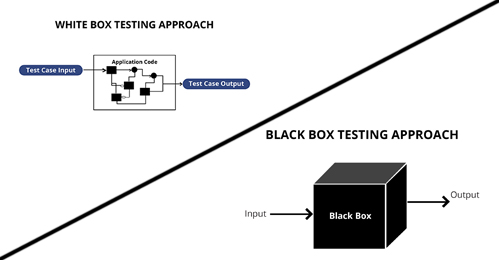
\includegraphics[scale=0.6]{assets/WhiteBoxBlackBoxTesting.jpg}
		\caption{Black-Box/White-Box Testing (Quelle: \textcite{khandelwal_difference_2019})}
		\label{fig:WhiteBoxBlackBoxTesting}
	\end{figure}
	
	
	\section{Test Driven Devlopment}
	\acfi{TDD} ist ein Konzept, bei dem Tests zuerst geschrieben werden und erst anschließend eine passende Implementierung erstellt wird die genau soviel beinhaltet, dass der Test erfolgreich durchgeführt werden kann.
	\ac{TDD} bietet daher mehrere Vorteile:
	
	\begin{itemize}
		\item Geschriebener Code kann überarbeitet oder verschoben werden, ohne dass die Gefahr besteht, Funktionalität zu beschädigen.
		\item Die Tests selbst werden durch die Implementierung getestet.
		\item Die Anforderungen können mit geringerem Aufwand umgesetzt werden, da nur die benötigte Funktion geschrieben wird.
	\end{itemize}

	\textcite{ammann_introduction_2016}
	
	\begin{figure}[ht]
		\centering
		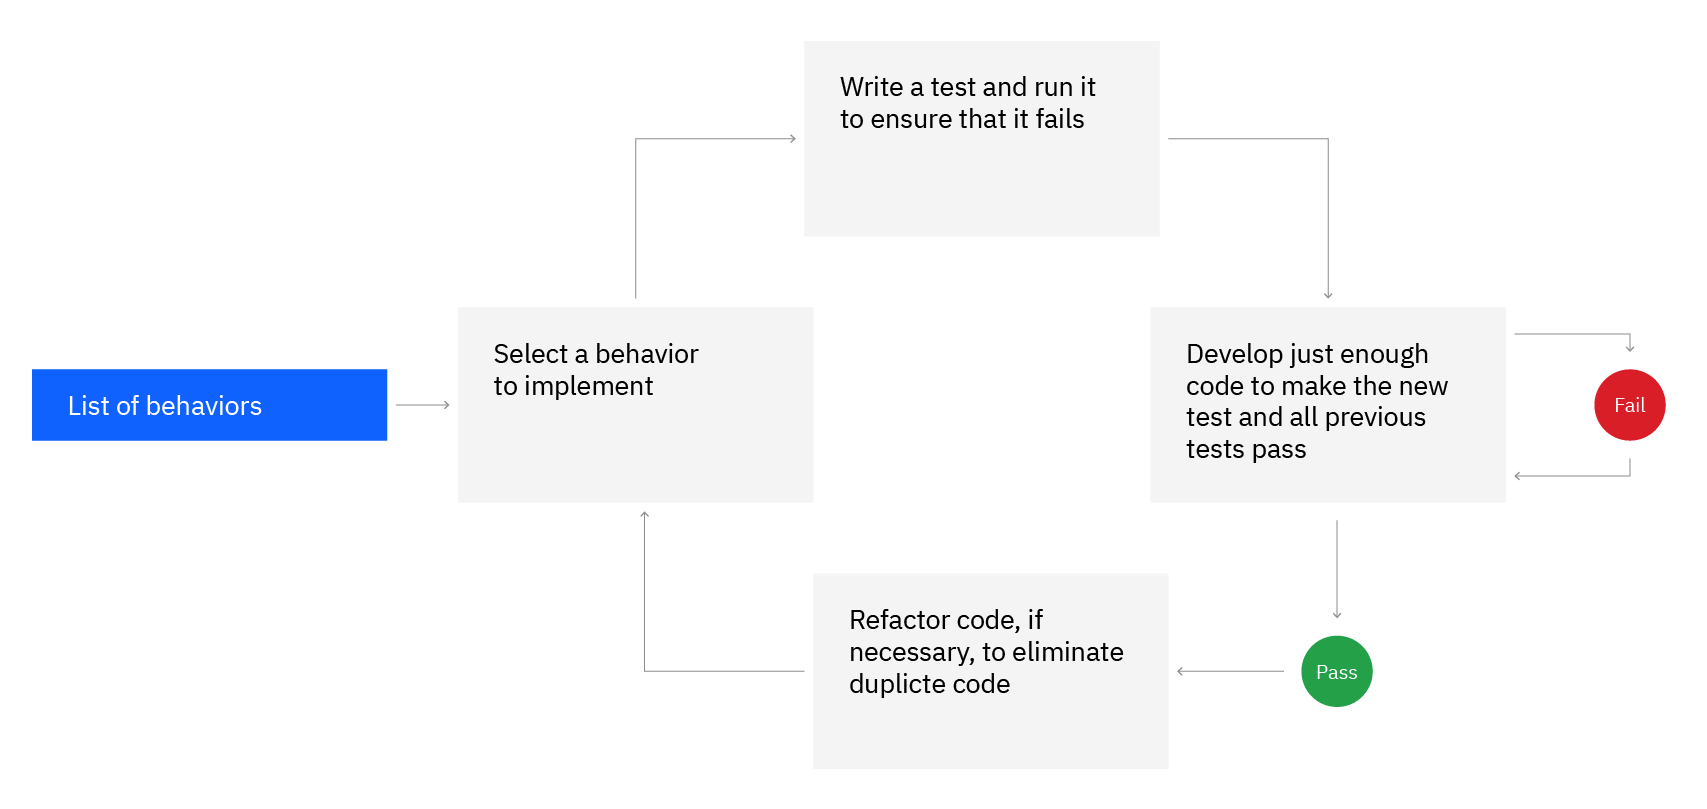
\includegraphics[scale=0.25]{assets/tdd-cycle.png}
		\caption{\acl{TDD} cycle (Quelle: \textcite{noauthor_test-driven_nodate})}
		\label{fig:tdd-cycle}
	\end{figure}
	
	\section{Test Case Management System} \label{sec:tcms}
	Ein \acl{TCMS} (\ac{TCMS}) ist eine Software, mit dem Test-Teams für ein bestimmtes Projekt oder eine Anwendung Testfälle verwalten, organisieren und analysieren können.
	Es hilft bei der Planung, Überwachung und Dokumentation von Tests und ermöglicht es, Testfälle sicher und effizient zu verwalten.
	
	Ein \ac{TCMS} ist ein wichtiges Werkzeug, um einen strukturierten und effektiven Testprozess zu gewährleisten und den Qualitätsstandard einer Anwendung zu verbessern.
	Es verfügt über Basisfunktionen wie Testfall-Erstellung, Testfall-Verwaltung, Testfall-Ausführung und Ergebnisberichterstattung. 
	Weiters kann ein solches System auch eine integrierte Umgebung für die Zusammenarbeit von verschiedene Abteilungen in einer Firma bereitstellen.
	
	Zusätzlich zu den Basisfunktionen sind weitere wichtige Merkmale:
	
	\begin{itemize}
		\item Attraktive Benutzeroberfläche und benutzerfreundliches Design
		\item Nachvollziehbarkeit
		\item verbesserte Zeitplanung und Organisation für Releases durch Reports
		\item Überwachung und Metriken
		\item Flexibilität
	\end{itemize}
	
	\textcite{lead_articles_nodate}	
	
	
	\subsection{Allgemeine Vorteile von Test Case Management Systemen}
	Einer der Hauptvorteile eines \ac{TCMS} besteht darin, dass sie den Testprozess verbessern. 
	Sie unterstützen auch die Kontrolle der Gesamtkosten, indem sie die Testautomatisierung nutzen, um einen reibungslosen Ablauf zu gewährleisten.  
	
	Einige Vorteile von \ac{TCMS} bezüglich der Testausführungsläufe sind:
	
	\begin{itemize}
		\item Sie geben einen besseren Überblick über das zu testende System, halten den gesamten Prozess auf Kurs und koordinieren die Testaktivitäten.
		\item Sie helfen bei der Feinabstimmung des Testprozesses, indem sie die Zusammenarbeit, Kommunikation und Auswertung unterstützen.
		\item Sie dokumentieren Aufgaben, Fehler und Testergebnisse und vereinfachen den Prozess, indem sie alles in einer einzigen Anwendung erledigen.
		\item Sie sind skalierbar und können eingesetzt werden, wenn die Testaktivitäten umfangreicher und komplexer werden.
	\end{itemize}

	\textcite{lead_articles_nodate}
	
	\subsection{Überblick von bestehenden Test Case Management Systeme}
	Auf dem Markt gibt es eine Vielzahl fertiger und direkt verwendbaren \ac{TCMS}, die die Verwaltung von Tests vereinfacht.
	
	Einige bekannte \ac{TCMS} sind:
	
	\begin{itemize}
		\item \textcite{noauthor_testrail_2023} 
		
		Webbasiertes \ac{TCMS}, ist zentralisiert und hat folgende Features:
		
		\begin{itemize}
			\setlength\itemsep{-0.5em}
			\item Test Planung, Verwaltung und Ausführung 
			\item Echtzeit Berichterstattung und Analysen
			\item Rückverfolgbarkeits- und Abdeckungsberichte für Anforderungen, Tests und Fehler
		\end{itemize}
		
		\item \textcite{noauthor_tricentis_nodate} 
		
		Webbasiertes \ac{TCMS} und hat folgende Features:
		
		\begin{itemize}
			\setlength\itemsep{-0.5em}
			\item Test Planung, Verwaltung und Ausführung 
			\item Echtzeit Test Status Update
			\item Berichterstattung
		\end{itemize}
		
		\item \textcite{noauthor_zephyr_nodate} 
		
		Webbasiertes \ac{TCMS}, kann in JIRA integriert werden und hat folgende Features:
		
		\begin{itemize}
			\setlength\itemsep{-0.5em}
			\item Test Planung, Verwaltung und Ausführung 
			\item Test Automatisierung
			\item Echtzeit Visualisierung von Projektstatus
		\end{itemize}
		
		\item \textcite{noauthor_tricentis_nodate-1} 
		
		Webbasiertes \ac{TCMS} und hat folgende Features:
		
		\begin{itemize}
			\setlength\itemsep{-0.5em}
			\item Test Planung, Verwaltung und Ausführung 
			\item Migrationsmöglichkeit von alten Test Management Lösungen
			\item Integrationsmöglichkeit mit Jenkins, Azure Pipelines, Bamboo oder jedem anderen CI/CD-Tool
			\item Anpassbare Dashboards, um über alle Releases, Projekte oder Programme im gesamten Unternehmen zu berichten
			\item Berichte per E-Mail oder URL teilen
		\end{itemize}
	\end{itemize}
	
	Welches Tool am besten geeignet ist, hängt natürlich von der jeweiligen Anwendung ab.
	\newline
	\begin{figure}[ht]
		\centering
		
\includegraphics[scale=0.5]{assets/best-tool-logos.jpg}
		\caption{Liste von aktuell führenden Test Case Management Systemen/Tools (Quelle: \textcite{noauthor_7_nodate})}
		\label{fig:tcms_logo}
	\end{figure}
	 
	
	\section{Verwendete Technologien} \label{sec:technologies}
	Dieser Abschnitt gibt eine Übersicht über die verwendeten Technologien, die für die Implementierung des in dieser Arbeit entwickelten \ac{TCMS} eingesetzt worden sind.
	
	\subsection{MariaDB}
	MariaDB ist eine weit verbreitete relationalen Open-Source-Datenbanken. 
	Sie wurde auf einem Fork von MySQL basierend von den ursprünglichen Entwicklern von MySQL entwickelt. 
	Der Fokus von MariaDB liegt auf Leistung, Stabilität und Offenheit. 
	Zu den jüngsten Erweiterungen gehören Clustering mit Galera Cluster 4, Kompatibilitätsfunktionen mit der Oracle-Datenbank und temporäre Datentabellen, mit denen Daten zu jedem beliebigen Zeitpunkt in der Vergangenheit abgefragt werden können.
	
	\textcite{noauthor_mariadb_nodate}
	
	\subsection{Docker}
	Docker ist eine Plattform mit der Entwickler einfach und schnell Container erstellen, bereitstellen, ausführen, aktualisieren und verwalten können.
	Container sind eigenständige, ausführbare Einheiten die unabhängig vom OS deployed werden können.
	Container vereinfachen die Entwicklung und Bereitstellung von verteilten Anwendungen. 
	Entwickler können Container auch ohne Docker erstellen doch Docker macht die Containerisierung schneller, einfacher und sicherer. 
	Telepresence ist die neuste Erweiterung und bietet einen einfachen Weg mit Kubernetes zu entwickeln.
	
	\textcite{ghosh_docker_2020}
	
	\begin{figure}[ht]
		\centering
		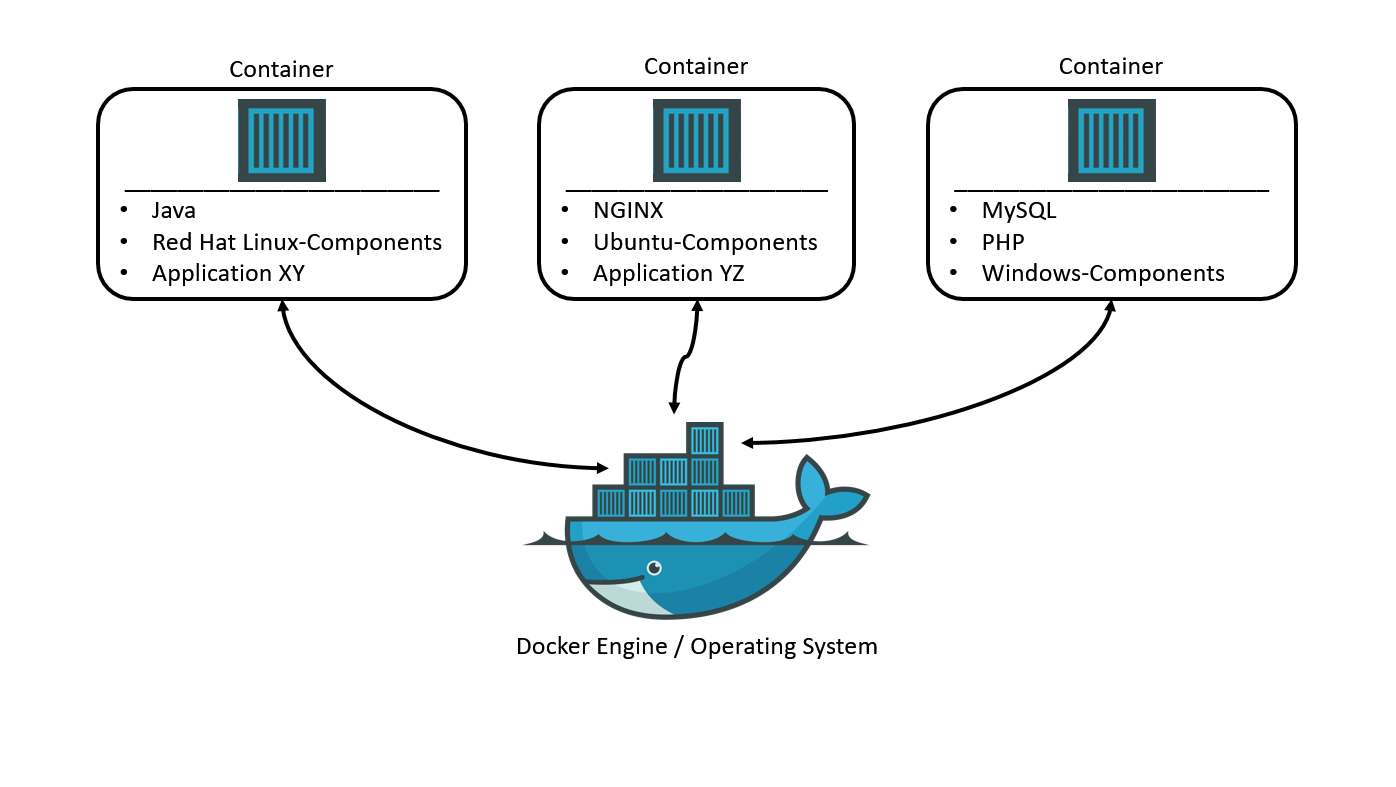
\includegraphics[scale=0.4]{assets/docker-funktionsweise.png}
		\caption{Funktionsweise von Docker (Quelle: \textcite{bollhoff_kubernetes_2022})}
	\end{figure}
	
	\subsection{Microsoft .NET Core} \label{subsec:msNetCore}
	Microsoft .NET Core ist ein Open-Source und plattformübergreifendes Framework um Applikationen auf Android, Apple, Linux und Windows Betriebssystemen zu entwickeln.
	Microsoft .NET Core unterstützt mehrere Programmiersprachen wie C\#, F\# und Visual Basic.
	Zudem bietet .NET einen Paketmanager um einfach und effizient Bibliotheken von Drittanbietern zu verwenden.
	Die neue Version .NET 8 bietet einige Neuerungen wie beispielsweise Performance-focused Typen, die die Leistung einer Anwendung erheblich verbessern soll.
	.NET 8 wird offiziell im November 2023 veröffentlicht.
	
	\textcite{billwagner_net_nodate}
	
	\subsection{Microsoft ASP.NET Core}
	Microsoft ASP.NET Core ist im Gegensatz zu .NET Core ein Framework um Webanwendungen zu entwickeln. 
	ASP.NET verfügt über Vorteile wie beispielsweise Blazor mit dem man einfach und effizient eine Interaktive Webbenutzeroberfläche mit C\# entwickeln kann.
	Dieses Framework unterstützt die Entwicklung und Implementierung von \acfi{API} und Mikroservices.
	Zudem ist ASP.NET laut \textcite{noauthor_techempower_nodate} schneller als jedes andere beliebte Web-Framework.
	
	\textcite{billwagner_net_nodate}
	
	\subsection{Entity Framework Core}
	\acfi{EF} Core ist eine \acfi{ORM} Technik für Microsofts .NET Core Technologie (\autoref{subsec:msNetCore}). 
	Die Technologie ist Open-Source, erweiterbar und plattformübergreifend.
	\ac{EF} Core unterstützt LINQ-Abfragen, Änderungsverfolgung, Aktualisierung sowie Schemamigration.
	Weiteres unterstützt \ac{EF} Core mehrere Datenbanken wie beispielsweise MySQL, PostgreSQL, Azure CosmosDB etc. und auch MariaDB.
	Die aktuelle Version von \ac{EF} Core ist 7.0 und verfügt über neue Funktionen wie z.B. das Mapping und Abfragen auf \acfi{JSON} Spalten. 
	Dabei ist es möglich einzelne Parameter von einem \ac{JSON} Objekt abzufragen und zu ändern.
	
	\begin{listing}[ht]
		\begin{minted}{csharp}
			var jeremy = await context
			.Authors
			.SingleAsync(author => author.Name.StartsWith("Jeremy"));
			
			jeremy.Contact = new() { 
				Address = new("2 Riverside", "Trimbridge", "TB1 5ZS", "UK"), 
				Phone = "01632 88346" 
			};
		
			await context.SaveChangesAsync();
		\end{minted}
		\caption{Update von einem Parameter einer \ac{JSON} Spalte}
	\end{listing}

	\textcite{billwagner_net_nodate}
	
	\subsection{OpenAPI}
	Die OpenAPI-Initiative hat die \acfi{OAS} entwickelt, die eine \ac{API} Beschreibung standardisiert.
	Die \ac{OAS} ist eine Sprache für \acfi{HTTP} \ac{API}s, durch diese \ac{API}s standardisiert beschrieben werden können. 
	Mithilfe von einem OpenAPI-Code-Generator (\textcite{noauthor_openapi_nodate-1}) kann direkt Client-Code für verschiedene Technologien wie z.B. Typescript generiert werden.
	
	\textcite{noauthor_openapi_nodate}
	
	
	\chapter{Anforderungen} \label{chapter:requiremnts}
	Der Hauptteil dieser Arbeit ist es ein funktionierendes \ac{TCMS} mit den genannten Technologien zu entwickeln.
	Dabei steht Zuverlässigkeit, Geschwindigkeit und Skalierbarkeit im Vordergrund.
	Zudem soll geachtet werden, dass Ressourcen bzw. Entitäten wie beispielsweise Testfälle für mehrere Testpläne verwendet werden können damit mehrfache Einträge in der Datenbank verhindert werden.
	
	Das zu entwickelnde \ac{TCMS} hat folgende Anforderungen:
	
	\begin{itemize}
		\setlength\itemsep{-0.5em}
		\item Produkt und Testsysteme beschreiben
		\item Features beschreiben
		\item Features zu einem Produkt zuordnen
		\item Testfälle beschreiben
		\item Testfälle zu einem Feature zuordnen
		\item Testimplementierungen beschreiben
		\item Testimplementierungen zu Testfällen und Testsysteme zuordnen
		\item Testläufe von Testimplementierungen zu einem Testsystem zuordnen
		\item Resultate von bestimmten Testläufen abzufragen
	\end{itemize}
	
	
	\section{Minimum Viable Product}
	Ein \acfi{MVP} ist ein minimal brauchbares Produkt. 
	Dabei handelt es sich um die erste funktionierte Iteration eines Produkts das nur Kernfunktionalitäten beinhaltet.
	In unserem Fall ist das ein Funktionierendes \ac{TCMS} backend von der Datenbank abfrage bis hin zur \ac{API} und sollte die oben angeführten Anforderung abdecken.
	
	Der Vorteil ist, dass das Produkt so schnell wie möglich zum Kunden gelangt und das Produkt Kundenfeedback bekommt.
	Die Kunden von dem zu entwickelnden \ac{TCMS} sind in diesem Fall die Mitarbeitenden der Firma Ganter Instruments.
	
	\textcite{alliance_what_2017}
	
	
	\section{Testen der Funktionalitäten}
	Damit der Kunde die Funktionalitäten des \ac{TCMS} auch oberflächlich Testen kann, wird ein Tool namens Swagger verwendet um ein Webbasiertes \acfi{UI} bereitzustellen.
	Swagger ist grundsätzlich ein Werkzeug mit denen Teams \ac{API}-Beschreibungen erstellen können.
	Zudem kann Swagger mithilfe des standardisiertem \ac{OAS} automatisch ein \ac{UI} generieren.
	
	\textcite{noauthor_api_nodate}
	
	\begin{figure}[ht]
		\centering
		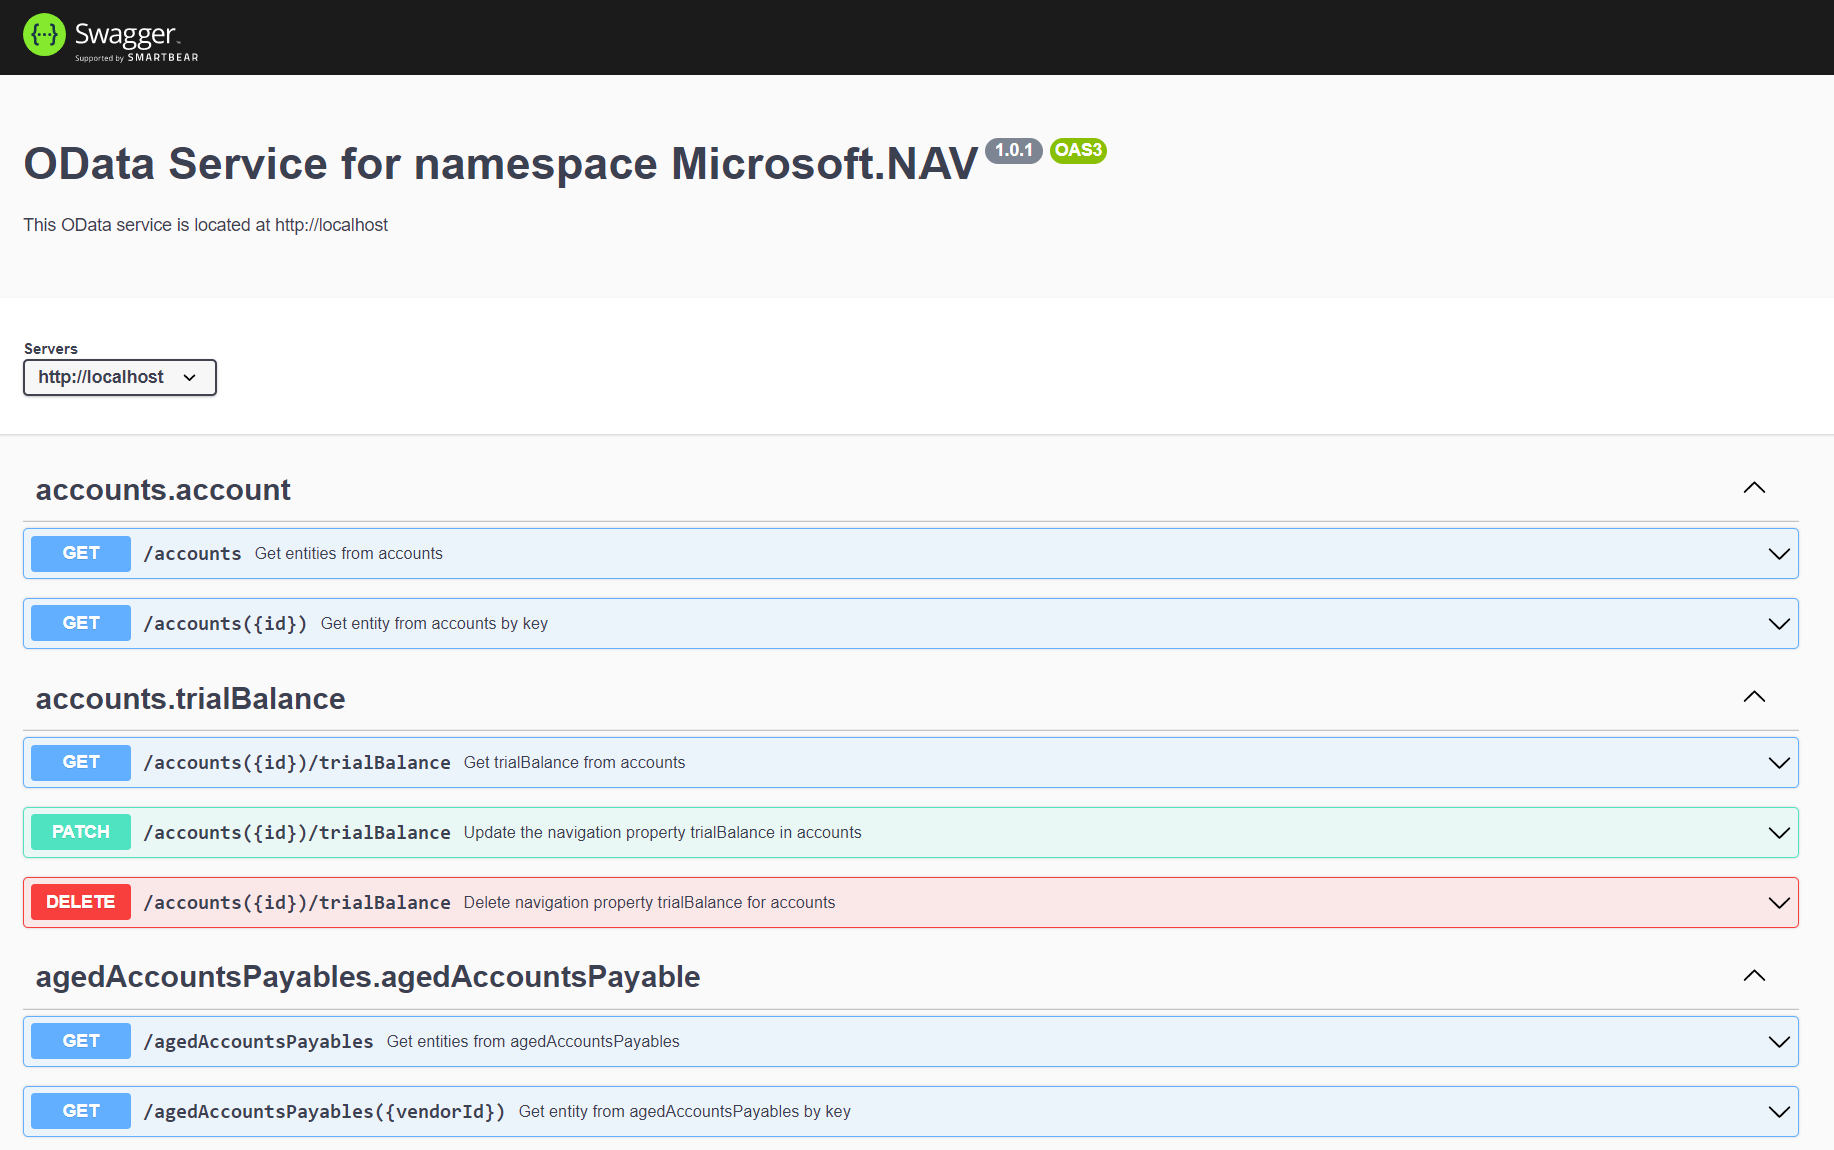
\includegraphics[scale=0.6]{assets/swaggerui.png}
		\caption{Beispiel \ac{UI} von Swagger (Quelle: \textcite{noauthor_host_nodate})}
	\end{figure}

	\section{Vorgehensweise} \label{sec:userStoriesDefinition}
	Damit das zu Entwickelnde \ac{TCMS} die eben genannten Anforderungen erfüllen kann werden diese in User-Stories aufgeteilt.
	Nachfolgend sind vier User-Stories aufgeführt, die erklären, welche Funktionalitäten das \ac{TCMS} beinhaltet, um die Anforderungen abzudecken.
	
	\subsection{Projekt und Datenbank Aufsetzen}
	Diese User Story beinhaltet noch keine Implementierung von Funktionalitäten, sondern beschäftigt sich mit dem Aufsetzten des Projektes und der Datenbank.
	
	Die Akzeptanzkriterien sind wie folgend:
	\begin{itemize}
		\item Projekt Struktur in die Architektur Schichten aufteilen 
		\item Datenbank mit Docker aufsetzen
		\item Datenbank manuell beschreibbar
	\end{itemize}
	
	\subsection{Erstellen und suchen von Test Environments}
	Als Nutzer:in möchte ich Test Environments erstellen und suchen, sodass ich Testpläne zuordnen kann.
	
	Die Akzeptanzkriterien sind wie folgend:
	\begin{itemize}
		\item Erstellen von Test Environments über Swagger \ac{UI}
		\item Suchen von Test Environments über Swagger \ac{UI}
		\item Hinzufügen und Entfernen von Testplänen über Swagger \ac{UI}
	\end{itemize}

	\subsection{Erstellen und suchen von Testplänen, Testfällen und Testimplementationen}
	Als Nutzer:in möchte ich Testpläne, Testfälle und Testimplementationen erstellen und suchen, sodass ich diese dementsprechend zuordnen kann.
	
	Die Akzeptanzkriterien sind wie folgend:
	\begin{itemize}
		\item Erstellen von Testplänen, Testfällen und Testimplementationen über Swagger \ac{UI}
		\item Suchen von Testplänen, Testfällen und Testimplementationen über Swagger \ac{UI}
	\end{itemize}
	
	\subsection{Erstellen und suchen von Testläufe}
	Als Nutzer:in möchte ich Testläufe erstellen und suchen, sodass ich Reports generieren kann.
	
	Die Akzeptanzkriterien sind wie folgend:
	\begin{itemize}
		\item Erstellen von Testläufen über Swagger \ac{UI}
		\item Suchen von Testläufen über Swagger \ac{UI}
	\end{itemize}
	
	
	
	\chapter{Konzept}
	Im vorherigen Kapitel wurden die Anforderungen des zu entwickelnden \ac{TCMS} festgelegt.
	Dieses Kapitel gibt nun einen Überblick über die Architektur, die dafür verwendet wird und vertieft sich in die Entwicklungsphasen des \ac{TCMS}.
	
	\section{Architektur}
	Grundlegend repräsentiert eine Softwarearchitektur die Organisation und den Aufbau eines Systems, zudem ist die Architektur eines der wichtigsten Komponente bei der Softwareentwicklung.
	Die Wahl der Softwarearchitektur ist zu Beginn eines Softwareprojektes sehr relevant, da diese hohen Einfluss auf den späteren verlauf des Projektes haben wird und es sehr kostenintensiv ist diese umzustellen.
	Eine gut strukturierte Software Architektur bringt dementsprechend einige Vorteile:
	
	\begin{itemize}
		%\setlength\itemsep{-0.5em}
		\item Übersichtlichkeit
		\item bessere Wartbarkeit
		\item Erweiterbarkeit
		\item Anpassungsfähigkeit
		\item Skalierbar
		\item reduziert kosten und verhindert Code Verdoppelung
		\item erhöht die Qualität der Software
		\item Hilf bei komplexen Problemstellungen
		\item reduziert den Time-to-Market Faktor durch effizienteres entwickeln
	\end{itemize}
	
	\textcite{richards_fundamentals_2020}
	
	\subsection{Backend} \label{subsec:backend}
	In dieser Arbeit haben wir uns für die Vierschichtigen \acfi{DDD} Architektur entschieden, da sich diese schon öfters bewährt hat und es gute Erfahrungen damit gab.
	Der Aufbau dieser Architektur unterteilt sich in vier Schichten:
	
	\begin{itemize}
		%\setlength\itemsep{-0.5em}
		\item Präsentationsschicht
		
		Diese Repräsentiert \ac{API}s, die reinkommende Anfragen entgegennimmt und dementsprechend Antworten liefert.
		Die Anfragen werden an die Applikationsschicht weitergeleitet.
		
		\item Applikationsschicht
		
		Diese Schicht interagiert mit der Präsentationsschicht und koordiniert Applikation Aktivitäten.
		Hier werden abhängig von den gelieferten Daten dementsprechende Domain Objekte erzeugt und der Infrastruktur weitergeleitet.
		
		\item Domainschicht
		
		Beinhaltet die Entitäten von der Domain und ist das Zentrum der Architektur.
		Diese Schicht wird von der Applikationsschicht und von der Infrastrukturschicht aufgerufen und beinhaltet die ganze Business-Logik.
		
		\item Infrastrukturschicht
		
		Hier wird mit der Applikationsschicht, der Domainschicht und der Datenbank interagiert.
	\end{itemize}

	\begin{figure}[ht]
		\centering
		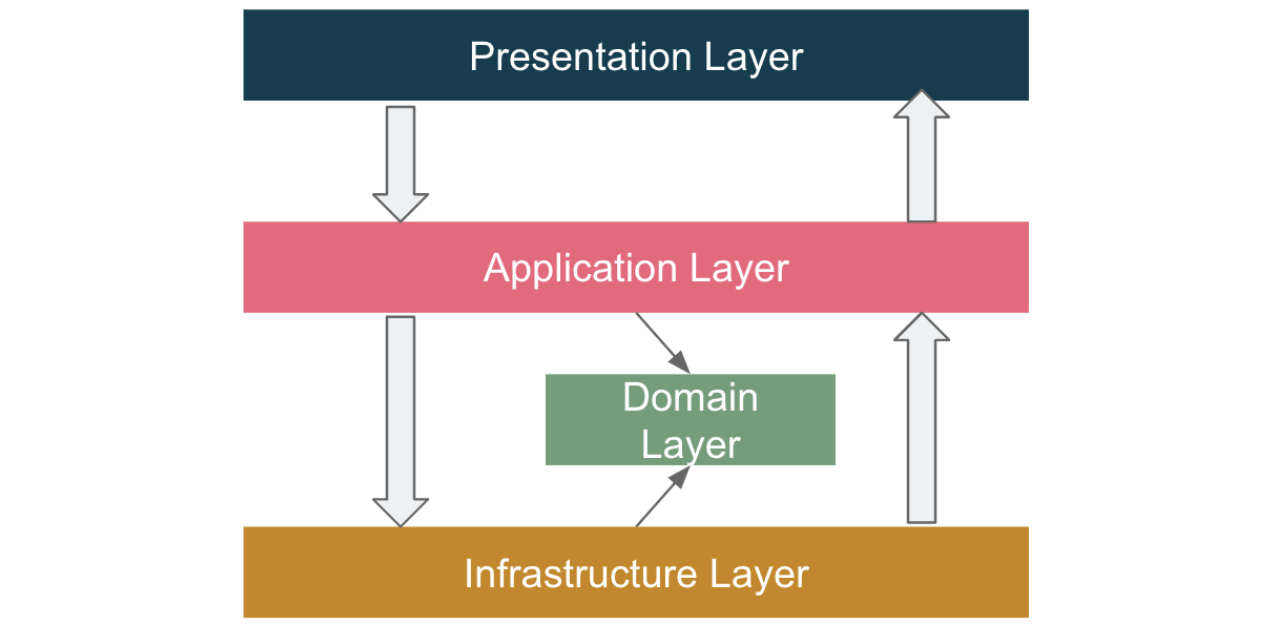
\includegraphics[scale=0.5]{assets/layeredArchitecture.png}
		\caption{Übersicht der Schichten (Quelle: \textcite{zhang_domain_nodate})}
	\end{figure}
	
	\ac{DDD} ist ein Design Ansatz, der sich auf den Input der Domainexperten konzentriert und somit die Entitäten des Systems dadurch modelliert werden.
	Das erleichtert es den Teammitgliedern, die Arbeit der anderen besser zu verstehen.
	Diese Verwendung trägt auch zur \emph{ubiquitous language} bei, die alle Teammitglieder bei Modell- und Entwurfsdiskussionen verwenden können.
	
	\textcite{vernon_implementing_2013}
	
	\begin{figure}[ht]
		\centering
		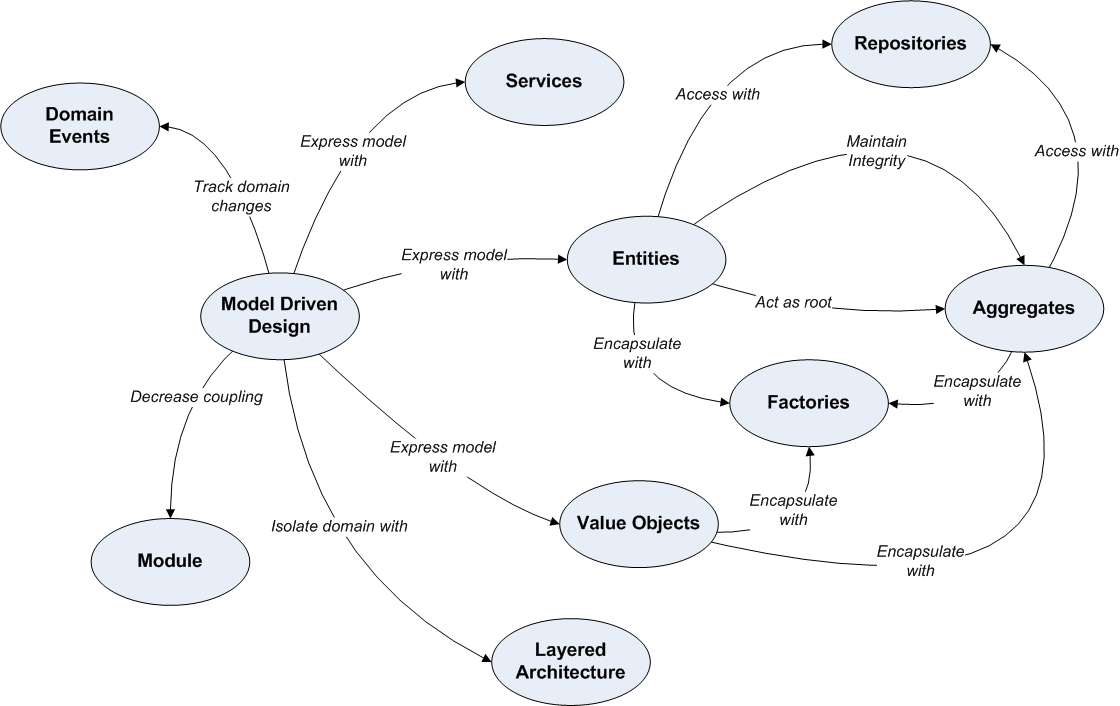
\includegraphics[scale=0.4]{assets/PatternsDDD.png}
		\caption{Komponenten von \ac{DDD} (Quelle: \textcite{noauthor_domain_nodate})}
	\end{figure}

	
	\section{Vorentwicklungsphase}
	In dieser Phase handelt es sich hauptsächlich um die Planung der Implementierung des \ac{TCMS}.
	Zuerst wurde eine Übersicht von dem schon bestehenden \acfi{TAS} erzeugt, das zeigt wie es mit dem \ac{TCMS} interagiert.
	Dabei greift das \ac{TAS} über die Technologie Automise über eine von \ac{TCMS} bereitgestellte \ac{API} darauf zu und erstellt Testläufe.
	Bei der Beschreibung von \autoref{fig:domainModelPart2} wird darauf genauer eingegangen (Siehe \autoref{subsec:domainModel}).
	
	\begin{figure}[ht]
		\centering
		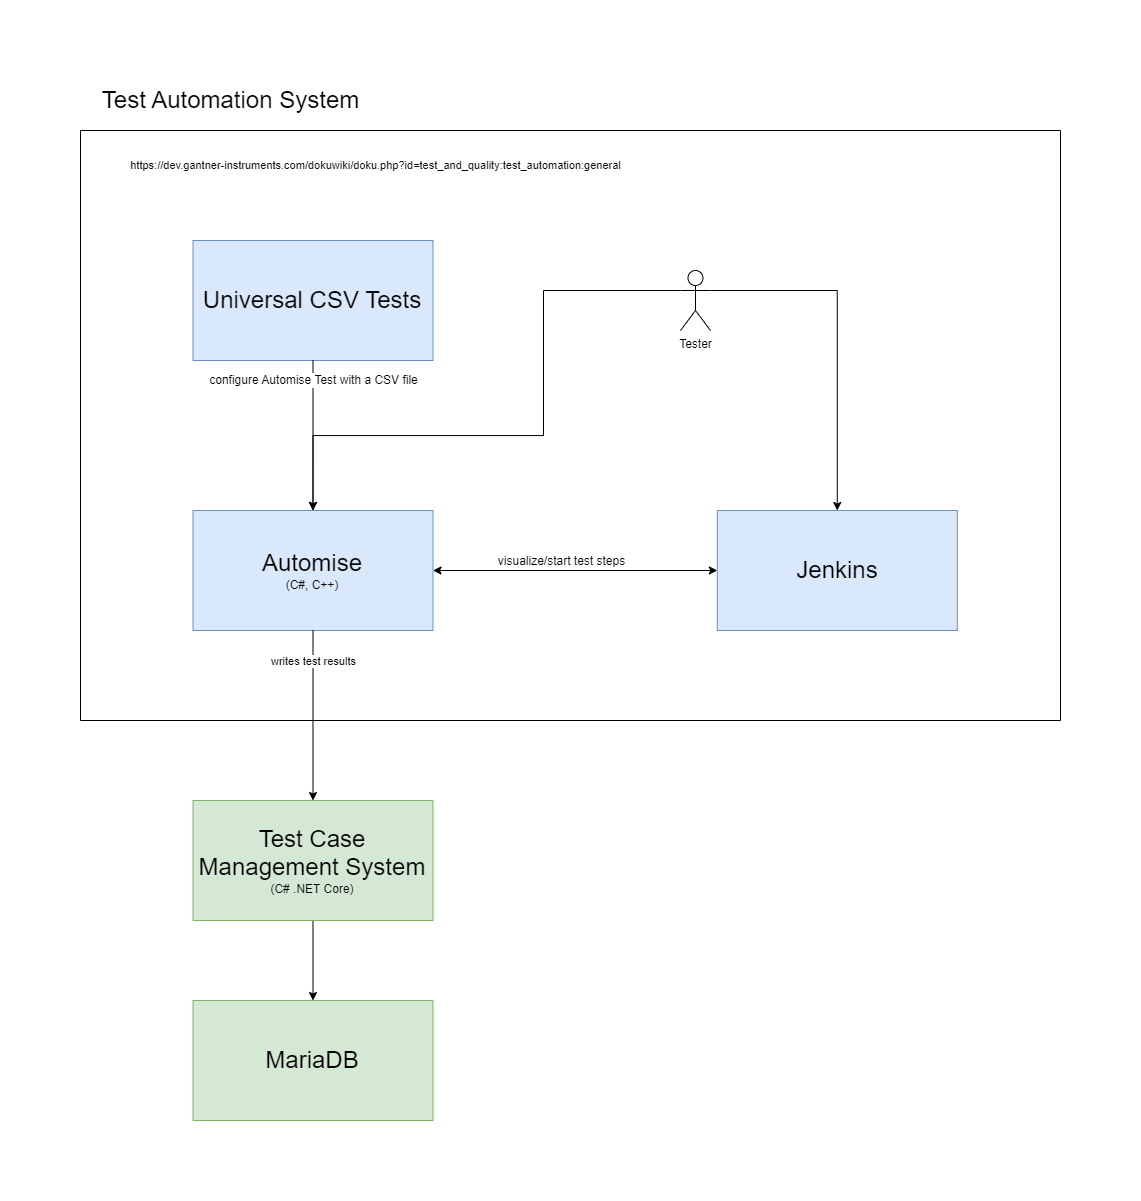
\includegraphics[scale=0.3]{assets/TestTechnologiesOverview.drawio.png}
		\caption{\ac{TAS} von \ac{GI}}
		\label{fig:testAutomationSystem}
	\end{figure}

	Durch die von \autoref{chapter:requiremnts} gegebenen Anforderungen und dem bestehendem \ac{TAS} wurde dementsprechend geplant.
	
	\subsection{Domain Model} \label{subsec:domainModel}
	Zunächst wurde das Domain-Model entwickelt, um die Entitäten und ihre Beziehungen darzustellen.
	Dabei wurden exakt, die von den Anforderungen geforderten Features abgebildet.
	
	\begin{figure}[ht]
		\centering
		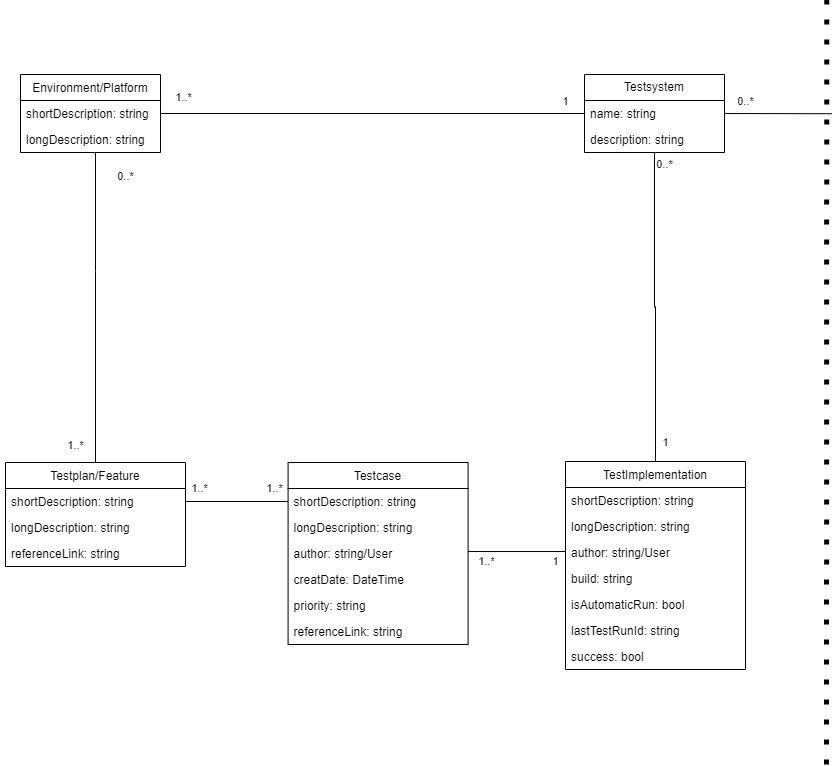
\includegraphics[scale=0.6]{assets/TCMS_DomainModel_part1.png}
		\caption{Domain-Model (Teil 1) aus den Anforderungen von \autoref{chapter:requiremnts}}
		\label{fig:domainModelPart1}
	\end{figure}

	Bei den in \autoref{fig:domainModelPart1} abgebildeten Entitäten handelt es sich um die folgenden Anforderungen:
	
	\begin{itemize}
		%\setlength\itemsep{-0.5em}
		\item Produkt und Testsysteme beschreiben
		
		Das Produkt wurde als Test Environment Entität modelliert, dass kann beispielsweise ein Gerät von der Firma sein.
		Das Testsystem bildet beispielsweise eine Prüfwand mit mehreren Geräten ab mit denen Tests durchgeführt werden.
		Jedes Produkt hat eigene Testsysteme.
		
		\item Features beschreiben
		
		Feature wurde als Testplan Entität modelliert.
		Ein Feature besteht aus mehreren Testfällen und bildet ein Feature von einem Gerät ab wie beispielsweise Netzwerk Connectivity.
		
		\item Features zu einem Produkt zuordnen
		
		Die erstellten Testpläne können nach dem Erstellen zu Test Environments zugeordnet werden.
		Somit können Testpläne für andere Environments wiederverwendet werden.
		
		\item Testfälle beschreiben
		
	    Ein Testfall besteht aus mehreren Testimplementationen.
	    Diese Testimplementationen sind für jeden Testfall unique und können nicht wiederverwendet werden. 
	    Ein Testfall ist beispielsweise eine überprüfung ob das Gerät eine \acfi{DHCP} Adresse erhalten hat.
		
		\item Testfälle zu einem Feature zuordnen
		
		Die Teställe können dann zu Features zugeordnet werden.
		Somit können Testfälle wiederverwendet werden.
		
		\item Testimplementierungen beschreiben
		
		Testimplementierungen sind grundsätzlich Beschreibungen wie ein Testfall getestet wird und ob dieser manuell oder automatisch ausgeführt wird.
		Testimplementierungen enthalten auch Informationen, ob sie Positiv beim letzten Testlauf getestet worden sind.
		Eine Testimplementation ist beispielsweise die Beschreibung mit welchen Konfigurationen ein Testfall bei einem Gerät getestet wird.
		
		\item Testimplementierungen zu Testfällen und Testsysteme zuordnen
		
		Testimplementierungen könne zu Testfällen und zu Testsysteme zugeordnet werden.
		Durch die Zuordnung von Testimplementierungen zu Testsystemen ist es einfacher die Testimplementierungen von einer Environment darzustellen.
		Somit kann beispielsweise ein Report generiert werden, der einen Überblick über jede Testimplementation von einem Environment gibt.
	\end{itemize}

	\begin{figure}[ht]
		\centering
		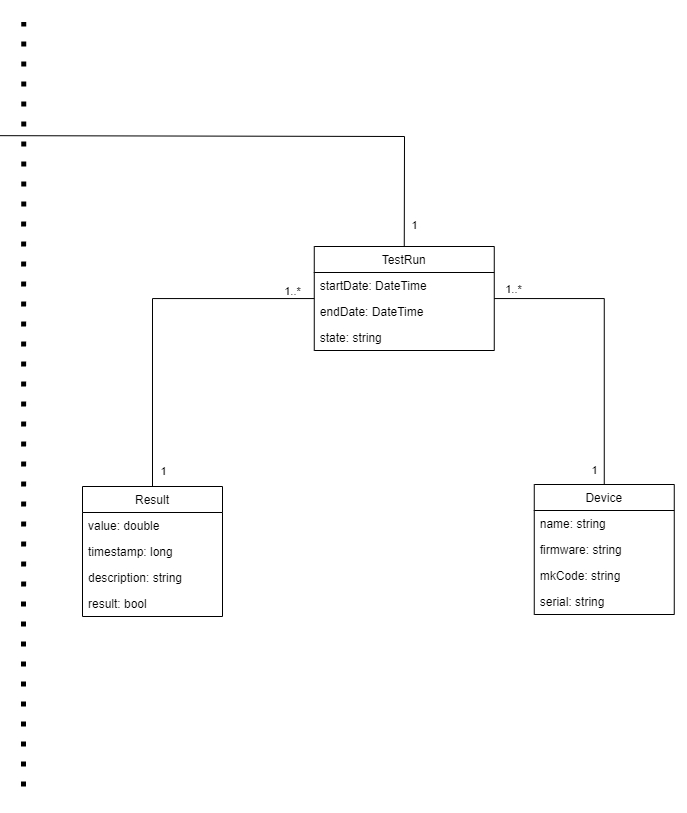
\includegraphics[scale=0.6]{assets/TCMS_DomainModel_part2.png}
		\caption{Domain-Model (Teil 2) aus den Anforderungen von \autoref{chapter:requiremnts}}
		\label{fig:domainModelPart2}
	\end{figure}

	Bei den in \autoref{fig:domainModelPart2} abgebildeten Entitäten handelt es sich um die folgenden Anforderungen:
	
	\begin{itemize}
		%\setlength\itemsep{-0.5em}
		\item Testläufe von Testimplementierungen zu einem Testsystem zuordnen
		
		Testläufe werden automatisch von dem bereits bestehenden \ac{TAS} der Firma erstellt und beschrieben.
		Diese Testläufe enthalten Informationen welche Testimplementationen, mit welchen Konfigurationen und mit welcher Hardware getestet wurde.
		Testläufe werden zum Zeitpunkt des Erstellens zu den jeweiligen Testsystemen zugeordnet, mit denen diese durchgeführt worden sind.
		
		\item Resultate von bestimmten Testläufen abzufragen
		
		Durch die Zuordnung von Testläufen zu Testsystemen können Resultate zu jedem Testsystem abgefragt werden.
	\end{itemize}
	
	Die in \autoref{fig:domainModelPart1} und \autoref{fig:domainModelPart2} gezeigten Entitäten wurden auf Basis der Kommunikation mit den Domainexperten so modelliert.
	
	\section{Datenbank Server}
	Der Datenbank Server wird mit Docker aufgesetzt.
	Über die bereitgestellten \ac{API}s des \ac{TCMS} wird dann über die schichten der verwendeten Architektur in die Datenbank geschrieben und gelesen werden (Siehe \autoref{subsec:backend}).
	Wie dies implementiert wird, wird im folgenden Kapitel beschrieben.
	
	
	\chapter{Technische Umsetzung}
	Damit das Ziel dieser Arbeit, ein \ac{TCMS} zu entwickeln, erreicht wird, werden die im \autoref{chapter:requiremnts} auf \autopageref{sec:userStoriesDefinition} definierten User-Stories mithilfe der erwähnten Technologien aus \autoref{sec:technologies} umgesetzt.
	Dabei wird auf den Scrum-Prozess und im Anschluss auf die User-Stories detailliert eingegangen.

	\section{Scrum}
	Scrum ist grundsätzlich eine Projektmanagement-Methode um in der Softwareentwicklung agil zu arbeiten.
	Bei dieser Methode geht es darum, dass ein Team Aufgaben von einer Aufgabenstellung in kleinen Schritten, sogenannte Sprints, angeht.
	
	\textcite{rubin_essential_2012}
	
	\begin{figure}[ht]
		\centering
		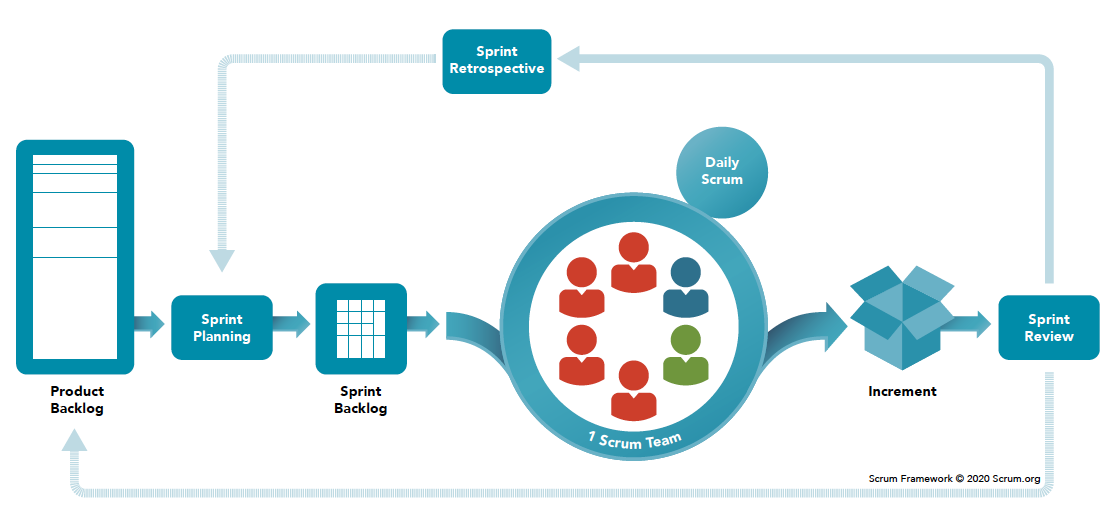
\includegraphics[scale=0.4]{assets/scrum-process.png}
		\caption{Scrum Prozess (Quelle: \textcite{noauthor_home_nodate})}
		\label{fig:scrum-process}
	\end{figure}
	
	Während der Implementierung des \ac{TCMS} dieser Arbeit wurde ein solcher Prozess angewendet (\autoref{fig:scrum-process}).
	
	\section{Implementierung der User-Stories}
	Dieser Abschnitt zeigt den Ablauf der Implementierung des \ac{TCMS} dieser Arbeit.
	Gesamt ist die Implementierung auf vier User-Stories aufgeteilt, die in folgender Reihenfolge implementiert wurden:
	
	\begin{itemize}
		\item Projekt und Datenbank Aufsetzen
		\item Erstellen und suchen von Test Environments
		\item Erstellen und suchen von Testplänen, Testfällen und Testimplementationen
		\item Erstellen und suchen von Testläufe
	\end{itemize}

	Zur Umsetzung des \ac{TCMS} kommt die Version .NET 7.0 zum Einsatz.
	Als \acfi{IDE} wurde \emph{Rider} verwendet, die von \emph{JetBrains} entwickelt wurde.

	\subsection{Projekt und Datenbank Aufsetzen}
	Damit eine Grundlage für die folgenden User-Stories vorhanden ist, wurde die Struktur des Projektes in vier Teil Projekte aufgeteilt.
	Dabei ist jedes Projekt die Projektion einer Schicht der verwendeten Architektur (Siehe: \autoref{subsec:backend}).
	
	Docker Desktop wurde für das Aufsetzen der Datenbank verwendet.
	Docker Desktop ist eine Anwendung die das Erstellen und Verwalten von Container einfacher macht.
	\autoref{lst:dockerDesktop} zeigt das Erstellen und Ausführen eines MariaDB Containers.
	
	\begin{listing}[ht]
		\begin{minted}{Basic}
			docker run --name mariadb-container 
			-e MYSQL_ROOT_PASSWORD=admin -p 3306:3306 -d mariadb:latest
		\end{minted}
		\caption{Starten eines MariaDB Containers}
		\label{lst:dockerDesktop}
	\end{listing}

	Nachdem der Container hochgefahren ist kann mit dem MariaDB Server gearbeitet werden.
	Weiters wurde ein Datenbankschema namens \emph{tcms\_mariadb} erstellt, wo die Tabellen abgespeichert werden (Siehe: \autoref{lst:createAndUseDBSchema}).
	
	\begin{listing}[ht]
		\begin{minted}{SQL}
			CREATE DATABASE tcms_mariadb; 
			USE tcms_mariadb;
		\end{minted}
		\caption{Erstellen und verwenden eines Datenbankschemas}
		\label{lst:createAndUseDBSchema}
	\end{listing}

	Um eine Verbindung zur Datenbank aufzustellen, liegt im Projekt ein \ac{JSON}-File, das die benötigten Konfigurationen bereitstellt (Siehe: \autoref{lst:connectionConfigs}).

	\begin{listing}[ht]
		\begin{minted}{JSON}
			{
				[...]
				
				"ConnectionStrings": {
					"MariaDbConnectionString": 
					"server=localhost;port=3306;database=tcms_mariadb;user=root;password=admin;"
				}
			}
		\end{minted}
		\caption{Konfigurationen für die Verbindung zur MariaDB Datenbank}
		\label{lst:connectionConfigs}
	\end{listing}

	Diese werden beim Start des Projektes in der \emph{Startup} Klasse gelesen und verwendet (Siehe: \autoref{lst:registerDatabase}).
	
	\begin{listing}[ht]
		\begin{minted}{csharp}
			[...]
			
			services.AddDbContext<EFContext>(dbContextOptions => {
				var connectionString = _config
					.GetConnectionString("MariaDbConnectionString");
					
				dbContextOptions
					.UseMySql(connectionString,
						ServerVersion.AutoDetect(connectionString));
			});
			
			[...]
		\end{minted}
		\caption{Ausschnitt der \emph{Startup} Klasse, der das Registrieren der Datenbank zeigt}
		\label{lst:registerDatabase}
	\end{listing}

	\autoref{lst:startupClassPart1}, \ref{lst:startupClassPart2} und \ref{lst:programClass} im Anhang auf Seite \autopageref{lst:startupClassPart1} zeigt die \emph{Startup} und \emph{Program} Klasse, die beim Start alles nötige initiiert.

	\subsection{Erstellen und suchen von Test Environments}
	\todo{Proper Erstellen und suchen von Test Environments Description}
	
	\subsection{Erstellen und suchen von Testplänen, Testfällen und Testimplementationen}
	\todo{Proper Erstellen und suchen von Testplänen, Testfällen und Testimplementationen Description}
	
	\subsection{Erstellen und suchen von Testläufe}
	\todo{Proper Erstellen und suchen von Testläufe Description}
	
	
	
	\chapter{Ergebnisse}
	\todo{Proper Ergebnisse Description}
	
	
	
	\chapter{Fazit und Ausblick}
	\todo{Proper Fazit und Ausblick}
	
	
	% Literaturverzeichnis
	\clearpage
	\phantomsection
	\addcontentsline{toc}{chapter}{Literaturverzeichnis}
	\printbibliography
	
	% Anhang
	\chapter*{Anhang}
	\addcontentsline{toc}{chapter}{Anhang}
	\begin{listing}[ht]
		\begin{minted}{csharp}
			public class Startup
			{
				private readonly IConfiguration _config;		
				
				public Startup(IConfiguration config) { _config = config; }
				
				// This method gets called by the runtime. 
				// Use this method to add services to the container.
				public void ConfigureServices(IServiceCollection services)
				{
					// Register database with the DI container
					services.AddDbContext<EFContext>(dbContextOptions => {
						var connectionString = _config
							.GetConnectionString("MariaDbConnectionString");	
									
						dbContextOptions
							.UseMySql(connectionString,
								ServerVersion.AutoDetect(connectionString));
					});
					
					// Register repositories with the DI container
					services.AddTransient<ITestCaseRepository, TestCaseRepository>();
					services.AddTransient<ITestPlanRepository, TestPlanRepository>();
					[...]
					
					// Register services with the DI container
					services.AddTransient<ITestCaseService, TestCaseService>();
					services.AddTransient<ITestPlanService, TestPlanService>();
					[...]
					
					services.AddControllers();
					services.AddSwaggerGen(c => { 
							c.SwaggerDoc("v1", 
								new OpenApiInfo { Title = "API", Version = "v1" }); 
					});
				}
				
			[...]
		\end{minted}
		\caption{\emph{Startup} Klasse Teil 1}
		\label{lst:startupClassPart1}
	\end{listing}

	\begin{listing}[ht]
		\begin{minted}{csharp}
			[...]
				
				// This method gets called by the runtime. 
				// Use this method to configure the HTTP request pipeline.
				public void Configure(IApplicationBuilder app, IWebHostEnvironment env)
				{
					if (env.IsDevelopment())
					{
						app.UseDeveloperExceptionPage();
						app.UseSwagger();
						app.UseSwaggerUI(c => 
							c.SwaggerEndpoint(
								"/swagger/v1/swagger.json", 
								"API v1"
							)
						);
					}
					
					app.UseHttpsRedirection();
					app.UseRouting();
					app.UseAuthorization();
					app.UseEndpoints(endpoints => { endpoints.MapControllers(); });
				}
			}
		\end{minted}
		\caption{\emph{Startup} Klasse Teil 2}
		\label{lst:startupClassPart2}
	\end{listing}

	\begin{listing}[ht]
		\begin{minted}{csharp}
			public class Program
			{
				public static void Main(string[] args)
				{
					// Use this line of code when we are going production
					// CreateHostBuilder(args).Build().Run();
					
					// Remove the code block below when we are going production
					var host = CreateHostBuilder(args).Build();	
					using (var scope = host.Services.CreateScope())
					{
						var services = scope.ServiceProvider;
						var dbContext = services.GetRequiredService<EFContext>();
						dbContext.Database.EnsureDeleted();
						dbContext.Database.EnsureCreated();
					}
					
					host.Run();
				}
				
				private static IHostBuilder CreateHostBuilder(string[] args)
				{
					return Host
						.CreateDefaultBuilder(args)
						.ConfigureWebHostDefaults(webBuilder => { 
							webBuilder.UseStartup<Startup>(); 
						});
				}
			}
		\end{minted}
		\caption{\emph{Program} Klasse, die die \emph{Startup} Klasse verwendet}
		\label{lst:programClass}
	\end{listing}

	\begin{listing}[ht]
		\begin{minted}{csharp}
			public class EFContext : DbContext
			{
				public DbSet<TestCase> TestCases { get; set; }
				public DbSet<TestPlan> TestPlans { get; set; }
				public DbSet<TestImplementation> TestImplementations { get; set; }
				public DbSet<TestRun> TestRuns { get; set; }
				public DbSet<TestEnvironment> TestEnvironments { get; set; }		
				public DbSet<TestSystem> TestSystems { get; set; }
				[...]
				
				public EFContext(DbContextOptions<EFContext> options) : base(options) { }	
				public EFContext() { }
				
				protected override void OnModelCreating(ModelBuilder modelBuilder)
				{
					base.OnModelCreating(modelBuilder);
					
					ApplyChildConfigurations(modelBuilder);
					
					modelBuilder.ApplyConfiguration(new TestCaseConfiguration());
					modelBuilder.ApplyConfiguration(new TestPlanConfiguration());
					modelBuilder.ApplyConfiguration(new TestImplementationConfiguration());
					modelBuilder.ApplyConfiguration(new TestRunConfiguration());
					modelBuilder.ApplyConfiguration(new TestEnvironmentConfiguration());
					[...]
				}
				
				private static void ApplyChildConfigurations(ModelBuilder modelBuilder)
				{
					modelBuilder.ApplyConfiguration(new TestSystemConfiguration());
					modelBuilder.ApplyConfiguration(new TestEnvironmentPlanConfiguration());
					[...]
				}
			}
		\end{minted}
		\caption{
			\emph{EFContext} Klasse, die \ac{EF} Core verwendet, um die Tabellen zu erstellen. 
			Diese Klasse wird, bei der Registrierung der Datenbank, in \autoref{lst:startupClassPart1} als Typ angegeben.
		}
		\label{lst:efcontextClass}
	\end{listing}
		
	\clearpage
	\section*{Eidesstattliche Erklärung}
	Ich erkläre hiermit an Eides statt, dass ich vorliegende Bachelorarbeit selbstständig und ohne Benutzung anderer als der angegebenen Hilfsmittel angefertigt habe. 
	Die aus fremden Quellen direkt oder indirekt übernommenen Stellen sind als solche kenntlich gemacht. 
	Die Arbeit wurde bisher weder in gleicher noch in ähnlicher Form einer anderen Prüfungsbehörde vorgelegt und auch noch nicht veröffentlicht.
	
	\vspace{3cm}
	\noindent
	Dornbirn, am \displaydate{date} \hfill Marco Prescher
	
	
\end{document}